% -------------------------------------------------------------------------------- %

\begin{exercise}

Ein bi-parental Heap (oder Beap) ist eine Datenstruktur, wo ein Knoten zwei Eltern hat (außer, es handelt sich um den ersten oder letzten Knoten auf einem Level) und zwei Kinder hat (außer, es ist ein Knoten am unstersten Level).

\begin{enumerate}[label = \alph*)]

  \item Sei $n$ die Anzahl der Knoten in einem Beap.
  Wie groß ist die Höhe des Beaps in etwa?
  Wie viele Elemente befinden sich auf dem letzten Level (unter der Annahme, dass dieser voll ist)?

  \item Betrachten wir nun einen MAX-Beap, d.h. einen Beap, bei dem die Einträge jedes Knotens größergleich den Einträgen in den Kindern dieses Knotens sind.
  Formulieren Sie einen Pseudocode für die Prozedur MAX-BEAPIFY, wobei das Feld $A$ und der Index $i$ gegeben sind, die Teil-Beaps mit den Wurzeln LEFT[$i$] und RIGHT[$i$] MAX-Beaps sind, der Eintrage $A[i]$ aber möglicherweise kleiner als die Einträge in den Kindern sein kann.

\end{enumerate}

\end{exercise}

% -------------------------------------------------------------------------------- %


\begin{solution}

Folgendes Bild ist in (inklusive rot vollständiger) Beap mit Indizierung, die die Datenfeld-Position des Elements angibt.

\begin{center}

  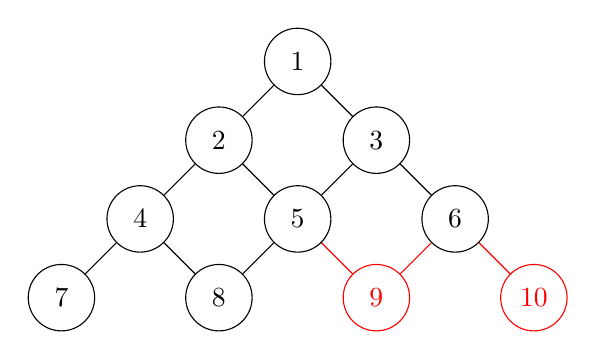
\begin{tikzpicture}

    \coordinate (x_1) at ( 0,  0);
    \coordinate (x_2) at (-1, -1);
    \coordinate (x_3) at ( 1, -1);
    \coordinate (x_4) at ( -2, -2);
    \coordinate (x_5) at ( 0, -2);
    \coordinate (x_6) at ( 2, -2);
    \coordinate (x_7) at (-3, -3);
    \coordinate (x_8) at (-1, -3);
    \coordinate (x_9) at (1, -3);
    \coordinate (x_10) at (3, -3);

    \draw [color = black] (x_1) -- (x_2);
    \draw [color = black] (x_1) -- (x_3);
    \draw [color = black] (x_2) -- (x_4);
    \draw [color = black] (x_2) -- (x_5);
    \draw [color = black] (x_3) -- (x_5);
    \draw [color = black] (x_3) -- (x_6);
    \draw [color = black] (x_4) -- (x_7);
    \draw [color = black] (x_4) -- (x_8);
    \draw [color = black] (x_5) -- (x_8);
    \draw [color = red]   (x_5) -- (x_9);
    \draw [color = red]   (x_6) -- (x_9);
    \draw [color = red]   (x_6) -- (x_10);

    \filldraw [color = black, fill = white] (x_1) circle (12 pt) node {$1$};
    \filldraw [color = black, fill = white] (x_2) circle (12 pt) node {$2$};
    \filldraw [color = black, fill = white] (x_3) circle (12 pt) node {$3$};
    \filldraw [color = black, fill = white] (x_4) circle (12 pt) node {$4$};
    \filldraw [color = black, fill = white] (x_5) circle (12 pt) node {$5$};
    \filldraw [color = black, fill = white] (x_6) circle (12 pt) node {$6$};
    \filldraw [color = black, fill = white] (x_7) circle (12 pt) node {$7$};
    \filldraw [color = black, fill = white] (x_8) circle (12 pt) node {$8$};
    \filldraw [color = red,   fill = white] (x_9) circle (12 pt) node {$9$};
    \filldraw [color = red,   fill = white] (x_10) circle (12 pt) node {$10$};

  \end{tikzpicture}

\end{center}

\begin{enumerate}[label = \alph*]

  \item Bezeichne also $n$ die Anzahl der Knoten, $h$ die Höhe und $k_i$ die Anzahl der Knoten auf dem $i$-ten Level, $i = 1, \dots, h$.
  Nehmen wir einmal an, dass das letzte Level voll ist.
  (Das ist bei der gegebenen Definition immer der Fall.)
  Wir sehen, dass, dass $k_i = i$.

  \begin{align*}
    n(h)
    =
    \sum_{i=1}^h i
    =
    \frac{h (h + 1)}{2}
    \iff
    h^2 + h - 2 n = 0
    \iff
    h(n)
    \stackrel{h > 0}{:=}
    -\frac{1}{2} + \sqrt{\frac{1}{4} + 2 n}
    =
    \frac{\sqrt{1 + 8 n} - 1}{2}
  \end{align*}


  Sei unser Beap mit $n$ Knoten nicht vollständig.
  Wir können den kleinsten vollständigen Ober-Beap mit $n^+ > n$ Knoten betrachten.
  Dieser hat klarerweise die selbe Höhe.
  Wir können aber auch den kleinsten vollständigen Unter-Beap mit $n^- < n$ Knoten betrachten.
  Dieser hat klarerweise eine Höhe weniger.

  \begin{multline*}
  h(n^-) + 1
  =
  \frac{\sqrt{1 + 8 n^-} - 1}{2} + 1
  \leq
  \frac{\sqrt{1 + 8 n} - 1}{2} \\
  \leq
  h(n)
  :=
  \ceil{\frac{\sqrt{1 + 8 n} - 1}{2}}
  =
  h(n^+)
  =
  \frac{\sqrt{1 + 8 n^+} - 1}{2}
  \end{multline*}

  In einem vollständigen Beap, mit $n$ Knoten, ist die Anzahl der Knoten im letzten Level genau $h(n)$.

  \item Wir orientieren uns an der Prozedur $\textsc{ErzeugeHalde}$ aus dem Skript.
  Wir nehmen also an, dass der Beap als Datenfeld realisiert ist und wir Identifizieren die Elemente mit ihrer Position in dem Datenfeld.
  Dabei gehen wir wie bei den Halden vor.
  Zunächst definieren wir uns eine Funktion sowie einige Prozeduren.


  \begin{align*}
    \textsc{Level}(i) := \ceil{\frac{\sqrt{1 + 8i} - 1}{2}},
    \quad
    \tilde h(i) := \frac{\sqrt{1 + 8 i} - 1}{2}
  \end{align*}

  Wir bezeichnen (sofern vorhanden) den rechten Elternteil als Vater, und den linken Elternteil als Mutter, sowie das rechte Kind als Sohn, und das linke Kind als Tochter.

  \phantom{}

  \begin{algorithmic}
    \Procedure{Mutter}{$i$}
      \If{$\textsc{Level}(i) - 1 = \tilde h(i - 1)$}
      \Comment Es gibt keine Mutter; das Element ist ganz links im Level.
        \State \Return $\NIL$
      \Else
          \State \Return $i - \textsc{Level}(i)$
      \EndIf
    \EndProcedure
  \end{algorithmic}

  \phantom{}

  \begin{algorithmic}
    \Procedure{Vater}{$i$}
      \If{$\textsc{Level}(i) = \tilde h(i)$}
        \Comment Es gibt keinen Vater; das Element ist ganz rechts im Level.
        \State \Return $\NIL$
      \Else
        \State \Return $i - \textsc{Level}(i) + 1$
      \EndIf
    \EndProcedure
  \end{algorithmic}

  \phantom{}

  \begin{algorithmic}
    \Procedure{Tochter}{$A, i$}
      \If{$i + \textsc{Level}(i) > A.\textit{HLänge}$}
        \Comment Es gibt keine Tochter.
        \State \Return $\NIL$
      \Else
        \State \Return $i + \textsc{Level}(i)$
        \EndIf
      \EndProcedure
  \end{algorithmic}

  \phantom{}

  \begin{algorithmic}
    \Procedure{Sohn}{$A, i$}
      \If{$i + \textsc{Level}(i) + 1 > A.\textit{HLänge}$}
        \Comment Es gibt keinen Sohn.
        \State \Return $\NIL$
      \Else
        \State \Return $i + \textsc{Level}(i) + 1$
      \EndIf
    \EndProcedure
  \end{algorithmic}

  \phantom{}

  \includegraphicsboxed{ ../../../Fundament-LaTeX/images/DGA/DGA - Algorithmus 22 - Extraktion des Maximums aus Prioritätswarteschlange}

  Nun können wir unsere Prozendur mittels $\textsc{AbwärtsKorrigieren}$ realisieren, wobei man die Prozedueren $\textsc{Links}$ und $\textsc{Rechts}$ durch $\textsc{Tochter}$ bzw. $\textsc{Sohn}$ ersetzen muss.

  \phantom{}

  \begin{algorithmic}
    \Procedure{Max-Beapify}{$A, i$}
      \State $A.\textit{HLänge} := A.\textit{Länge}$
      \State Vertausche $A[1]$ und $A[i]$
      \State $k := \textsc{Vater}(A.\textit{HLänge})$
      \If{$k = \NIL$}
        \State $k := \textsc{Mutter}(A.\textit{HLänge})$
      \EndIf
      \If{$\textsc{Level}(A.\textit{HLänge}) > 2$}
        \For{$j = k, \dots, 2$}
          \State $\textsc{AbwärtsKorrigieren}(A, j)$
        \EndFor
      \EndIf
    \EndProcedure
  \end{algorithmic}

\end{enumerate}

\end{solution}
